\chapter{Normal Burst Histograms}
\label{app:hists}

\par In Figures \ref{fig:app_hist_phib}--\ref{fig:app_hist_ap}, we present histograms showing the distributions of $\phi_B$, $a_B$, $\sigma_B$, $c$, $\phi_d$, $a_d$, $d$, $\lambda$, $\phi_p$ and $a_p$ we find in our population study of bursts in the Bursting Pulsar.  Each of these is a parameter we used to fit the Normal Bursts in our sample: see Section \ref{sec:struc} for a full explanation of these parameters.  In Figures \ref{fig:app_hist_phib_n}--\ref{fig:app_hist_ap_n} we show the distributions of $\phi_B$, $a_B$, $\phi_d$, $a_d$, $\phi_p$ and $a_p$ after being normalised by the persistent emission rate $k$ at the time of each burst.

\begin{figure}
  \centering
  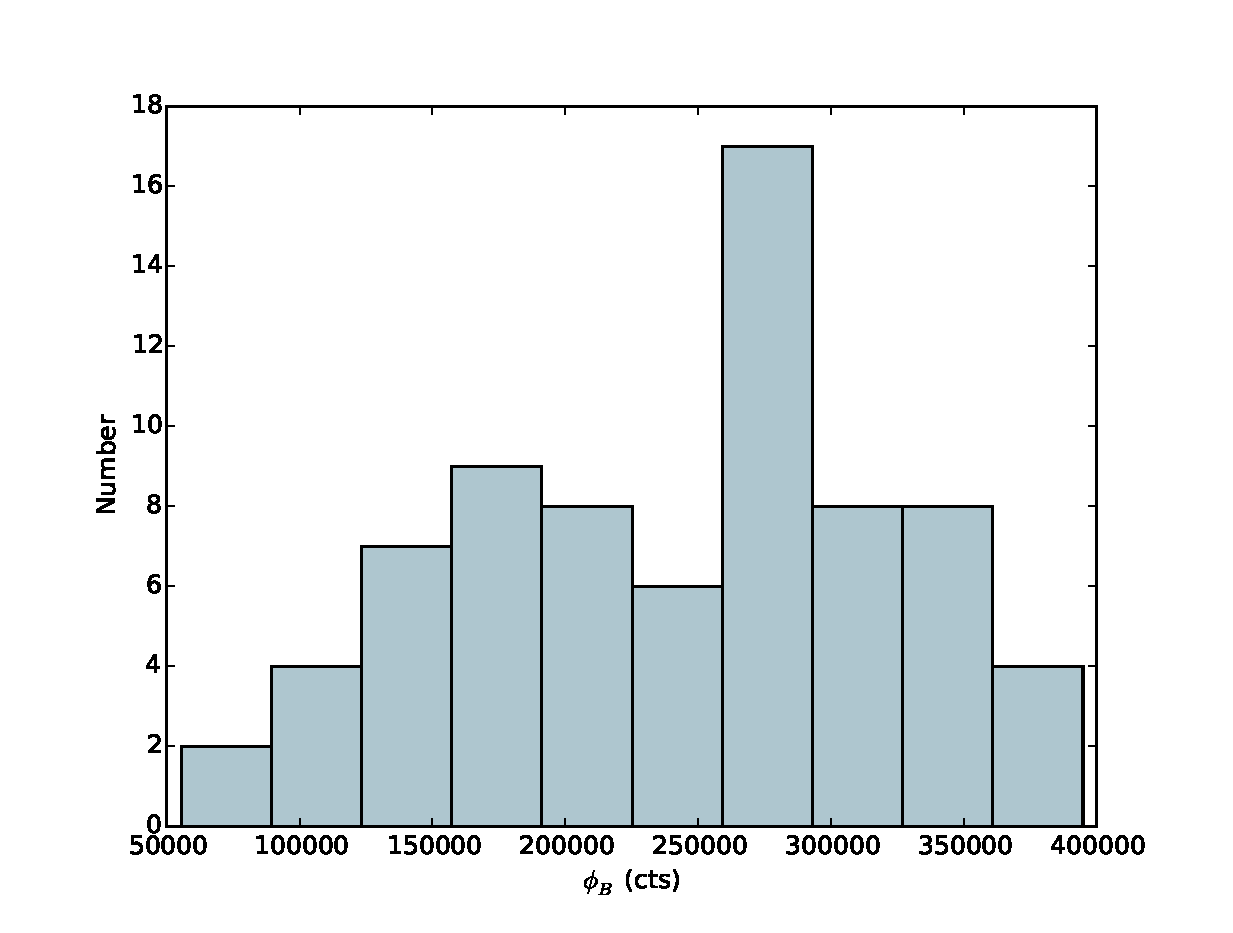
\includegraphics[width=.9\linewidth, trim={0cm 0 0cm 0},clip]{images/appendix_burst_aafluence_hist.eps}
  \caption{\small A histogram showing the distribution of burst fluence $\phi_B$ amongst our sample of Normal Bursts.}
  \label{fig:app_hist_phib}
\end{figure}

\begin{figure}
  \centering
  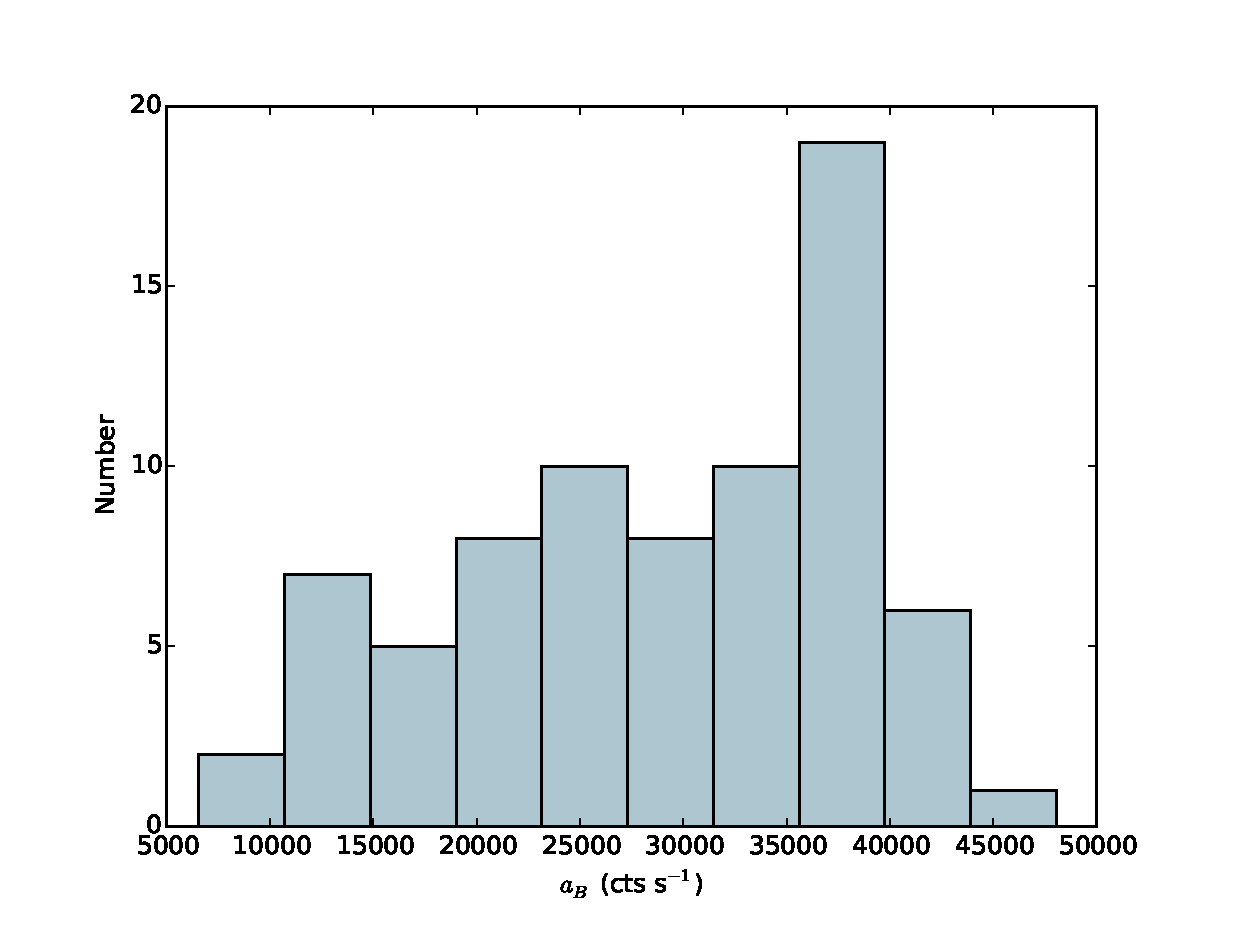
\includegraphics[width=.9\linewidth, trim={0cm 0 0cm 0},clip]{images/appendix_burst_pa_hist.eps}
  \caption{\small A histogram showing the distribution of burst amplitude $a_B$ amongst our sample of Normal Bursts.}
  \label{fig:app_hist_ab}
\end{figure}

\begin{figure}
  \centering
  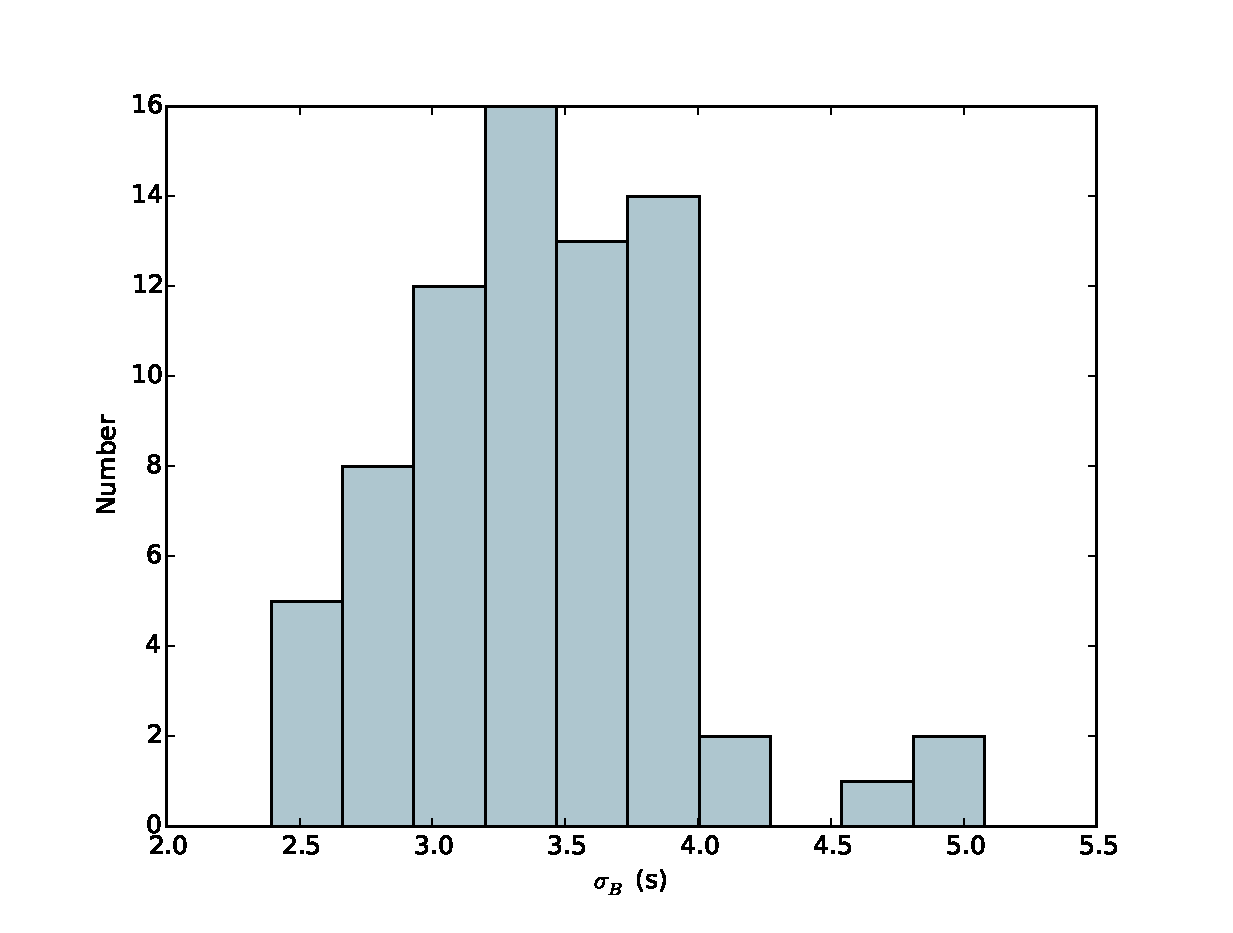
\includegraphics[width=.9\linewidth, trim={0cm 0 0cm 0},clip]{images/appendix_burst_sigma_hist.eps}
  \caption{\small A histogram showing the distribution of burst width $\sigma_B$ amongst our sample of Normal Bursts.}
  \label{fig:app_hist_sigb}
\end{figure}

\begin{figure}
  \centering
  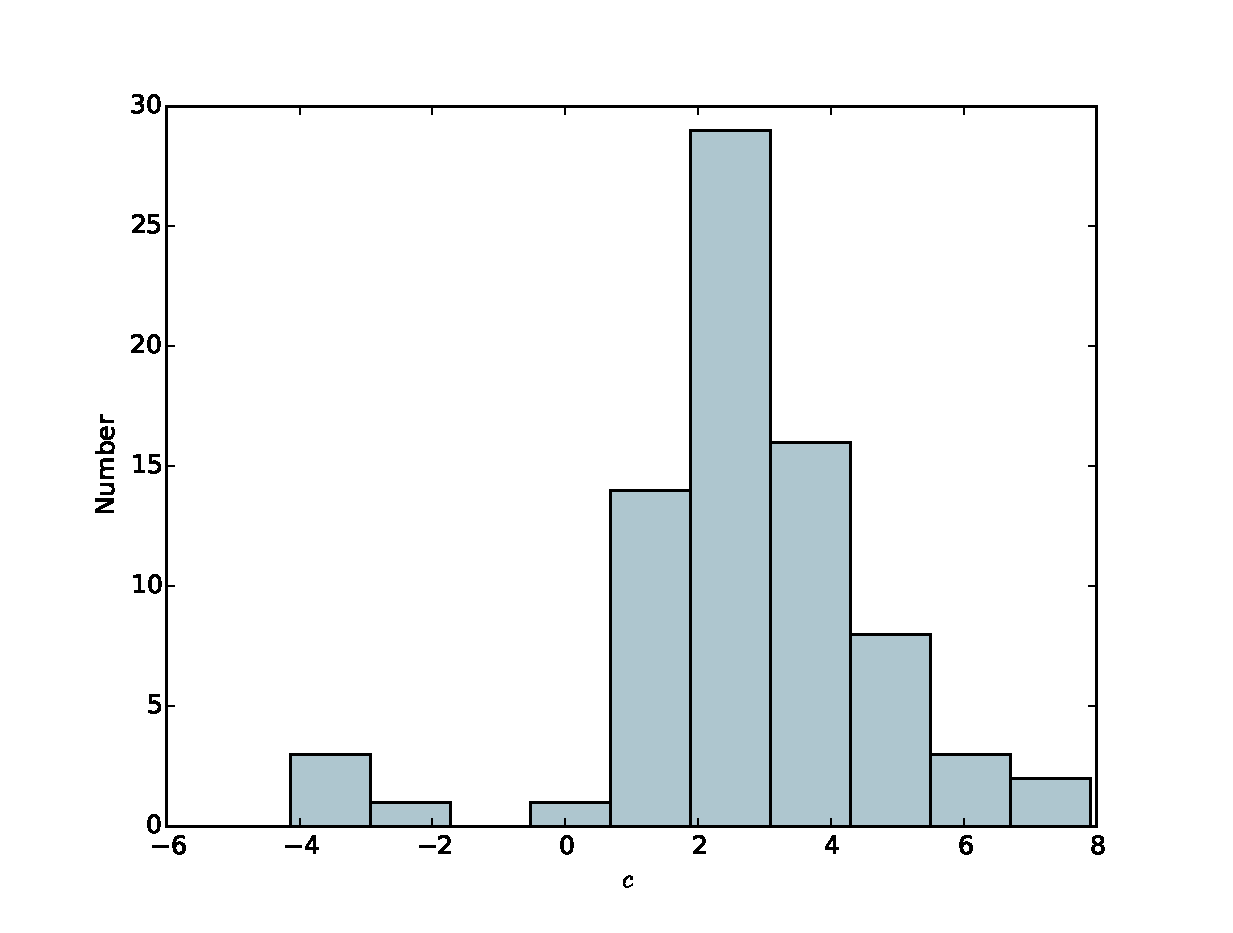
\includegraphics[width=.9\linewidth, trim={0cm 0 0cm 0},clip]{images/appendix_burst_skew_hist.eps}
  \caption{\small A histogram showing the distribution of burst skewness $c$ amongst our sample of Normal Bursts. }
  \label{fig:app_hist_c}
\end{figure}

\begin{figure}
  \centering
  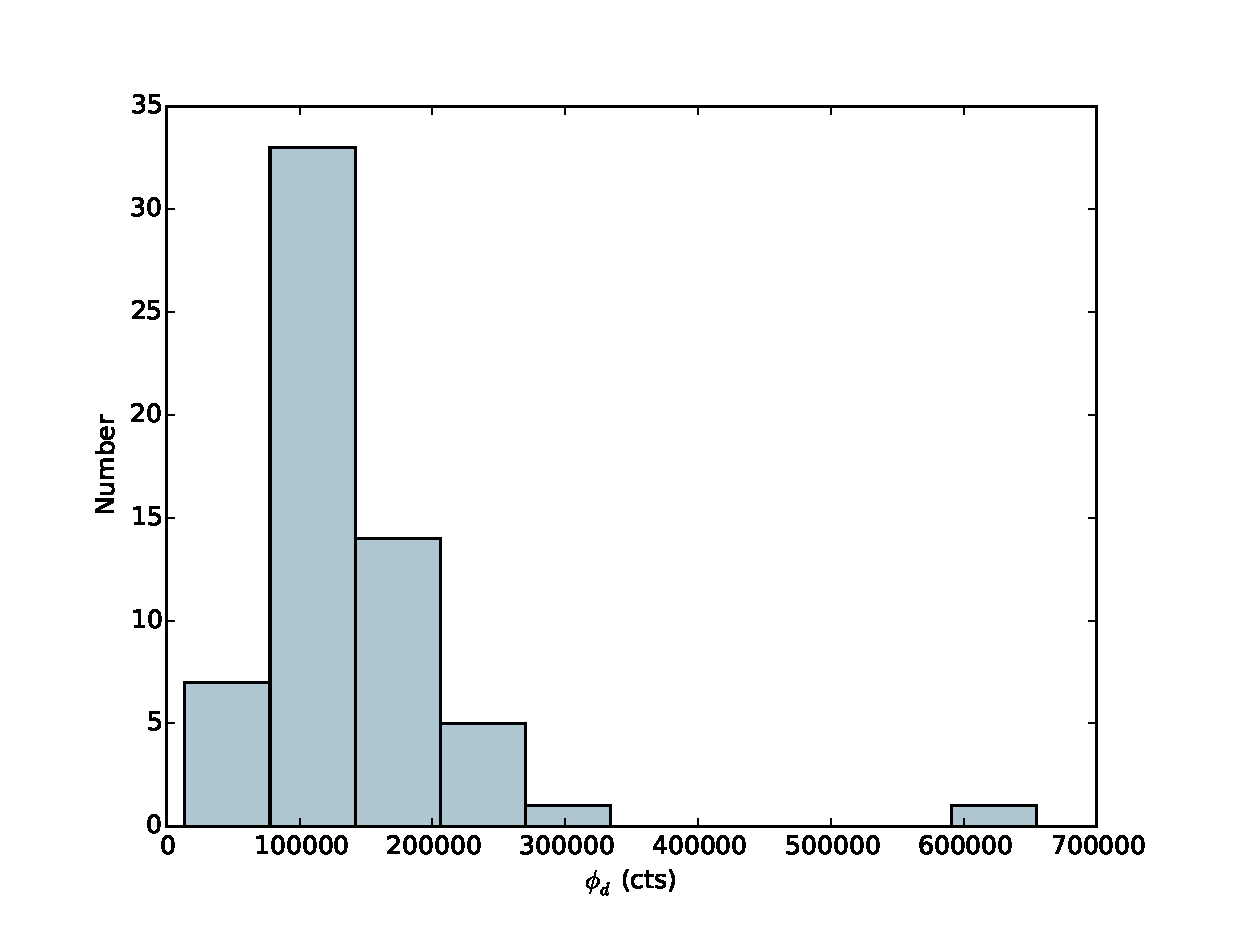
\includegraphics[width=.9\linewidth, trim={0cm 0 0cm 0},clip]{images/appendix_dip_aafluence_hist.eps}
  \caption{\small A histogram showing the distribution of dip fluence $\phi_d$ amongst our sample of Normal Bursts.}
  \label{fig:app_hist_phid}
\end{figure}

\begin{figure}
  \centering
  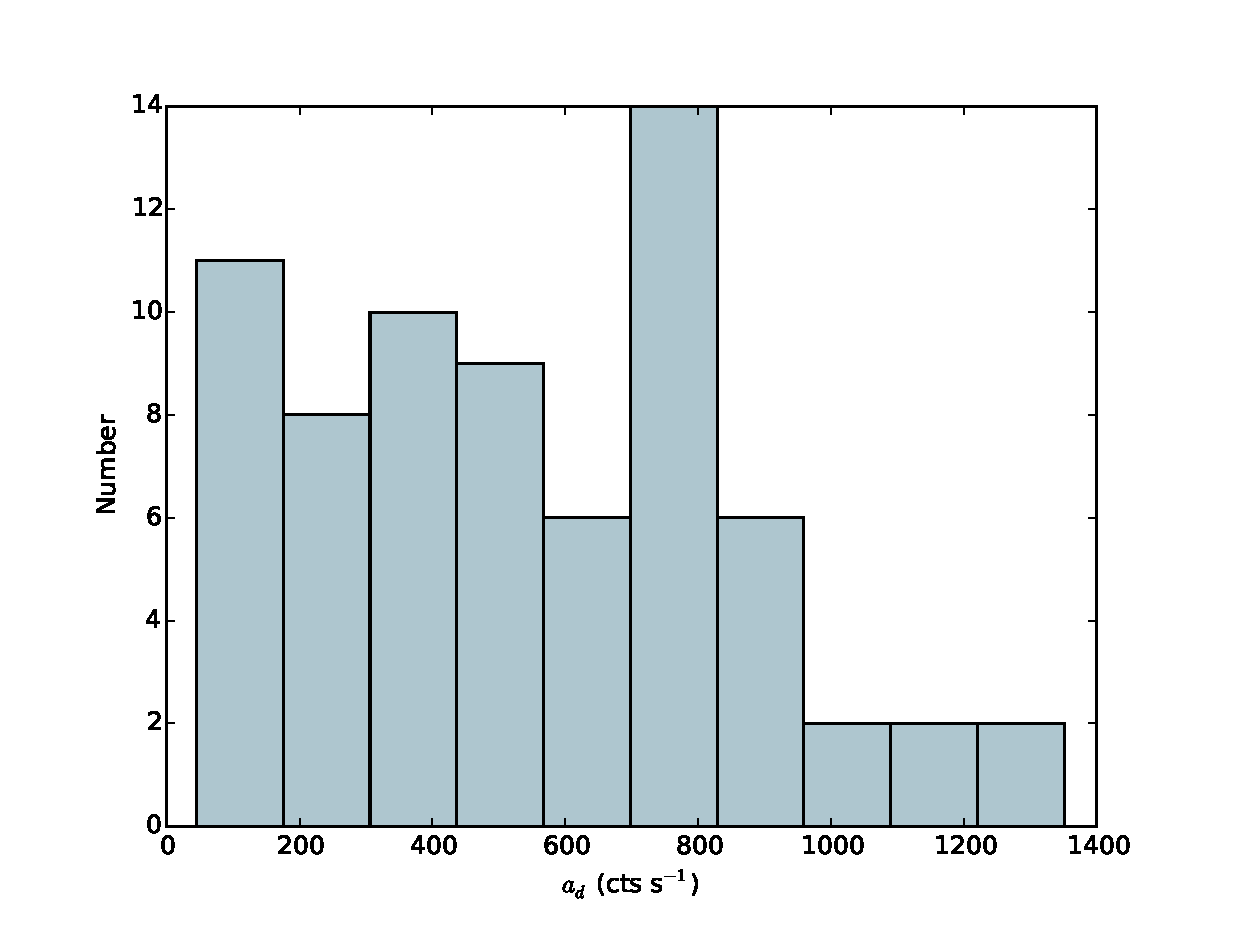
\includegraphics[width=.9\linewidth, trim={0cm 0 0cm 0},clip]{images/appendix_dip_pa_hist.eps}
  \caption{\small A histogram showing the distribution of dip amplitude $a_d$ amongst our sample of Normal Bursts.}
  \label{fig:app_hist_ad}
\end{figure}

\begin{figure}
  \centering
  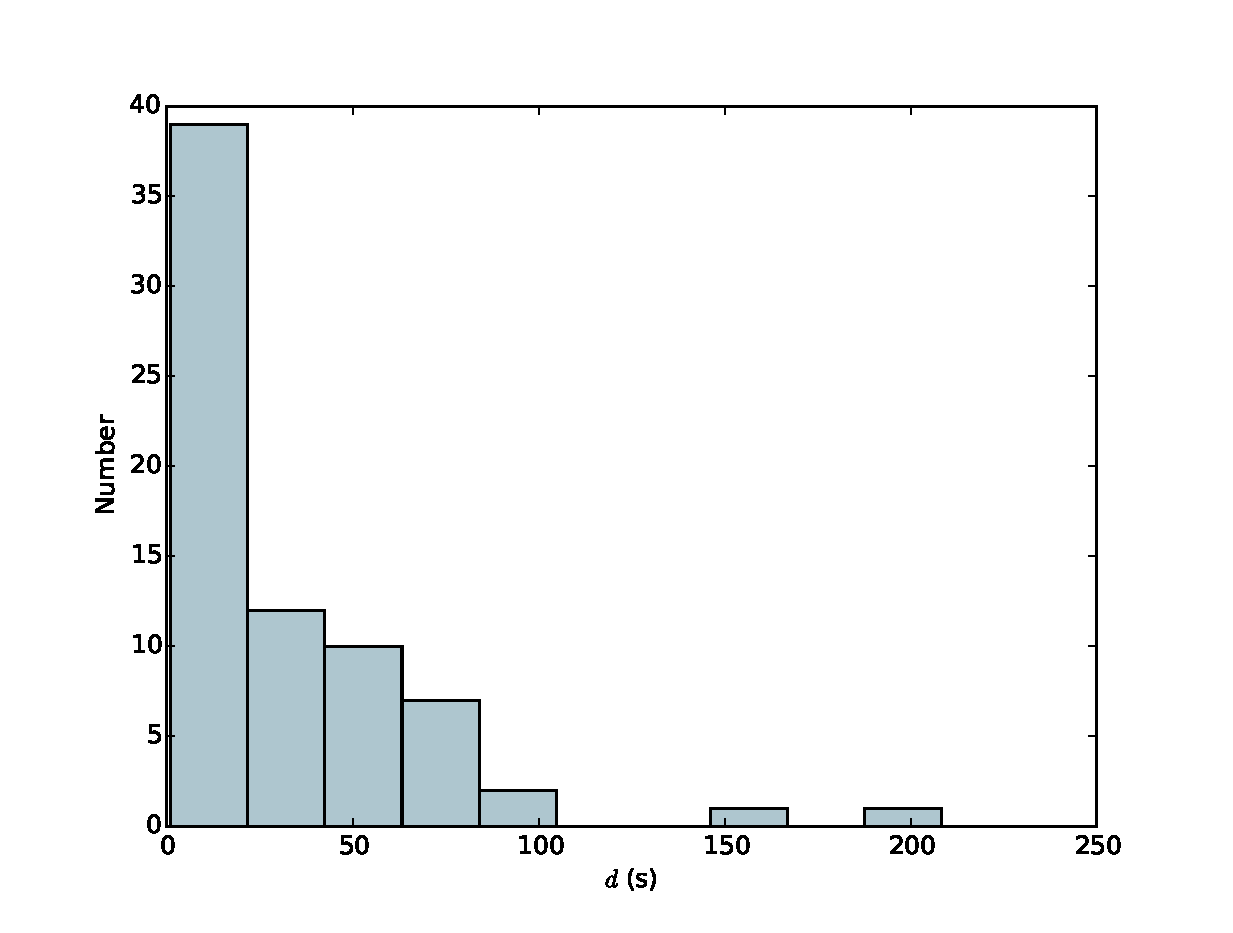
\includegraphics[width=.9\linewidth, trim={0cm 0 0cm 0},clip]{images/appendix_div_hist.eps}
  \caption{\small A histogram showing the distribution of dip fall-time $d$ amongst our sample of Normal Bursts.}
  \label{fig:app_hist_d}
\end{figure}

\begin{figure}
  \centering
  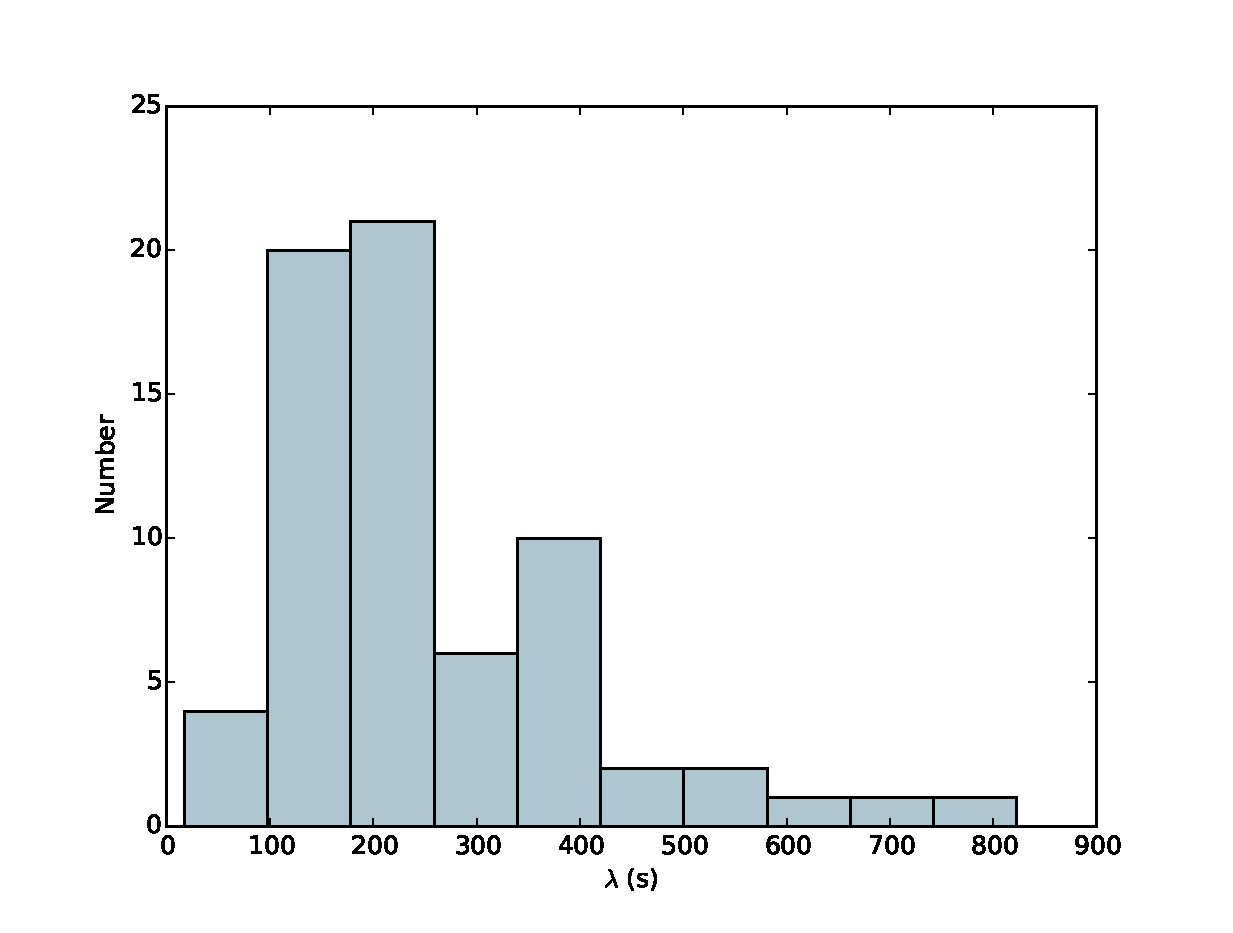
\includegraphics[width=.9\linewidth, trim={0cm 0 0cm 0},clip]{images/appendix_lambda_hist.eps}
  \caption{\small A histogram showing the distribution of dip recovery timescale $\lambda$ amongst our sample of Normal Bursts.}
  \label{fig:app_hist_lamb}
\end{figure}

\begin{figure}
  \centering
  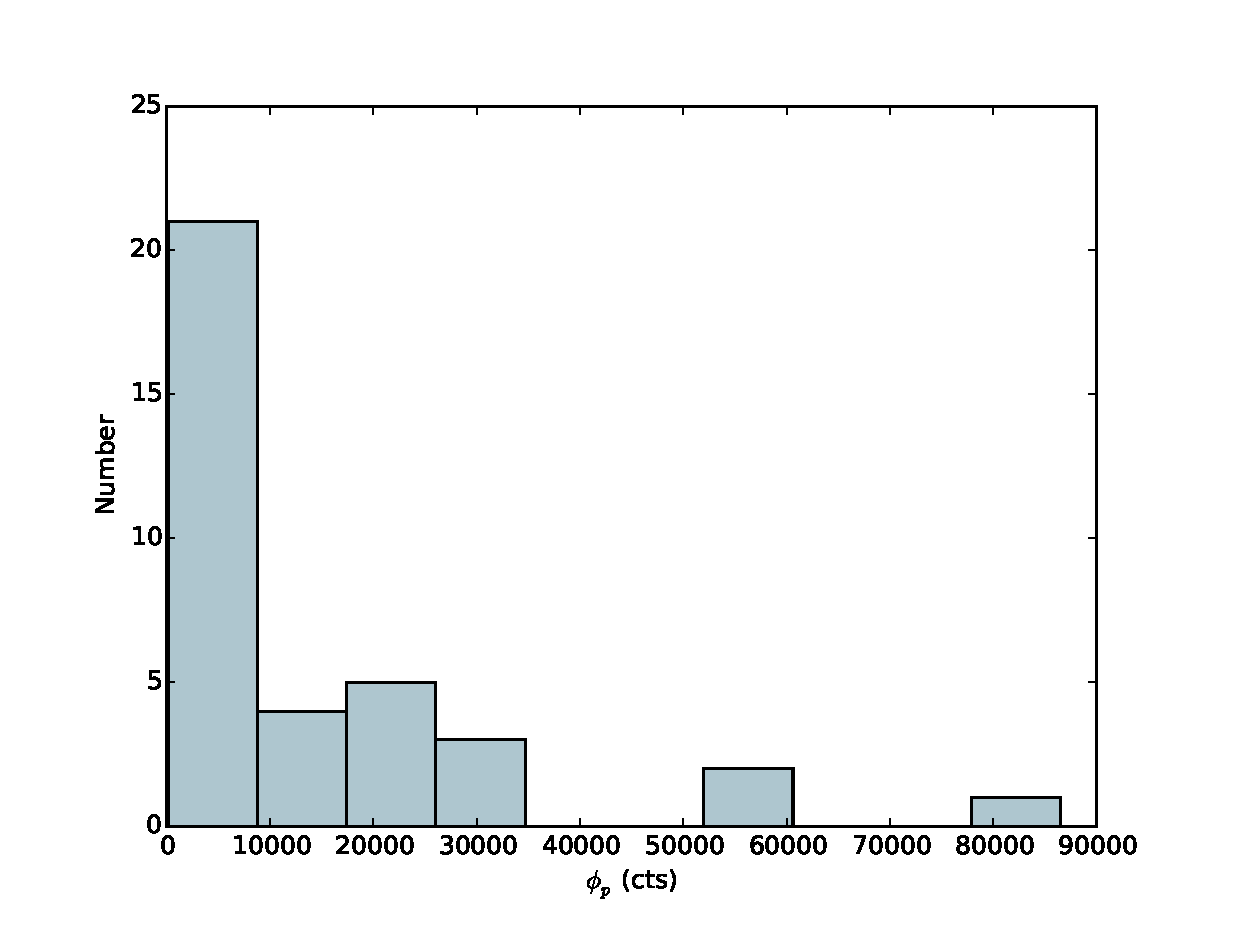
\includegraphics[width=.9\linewidth, trim={0cm 0 0cm 0},clip]{images/appendix_plat_aafluence_hist.eps}
  \caption{\small A histogram showing the distribution of plateau fluence $\phi_p$ amongst our sample of Normal Bursts.}
  \label{fig:app_hist_phip}
\end{figure}

\begin{figure}
  \centering
  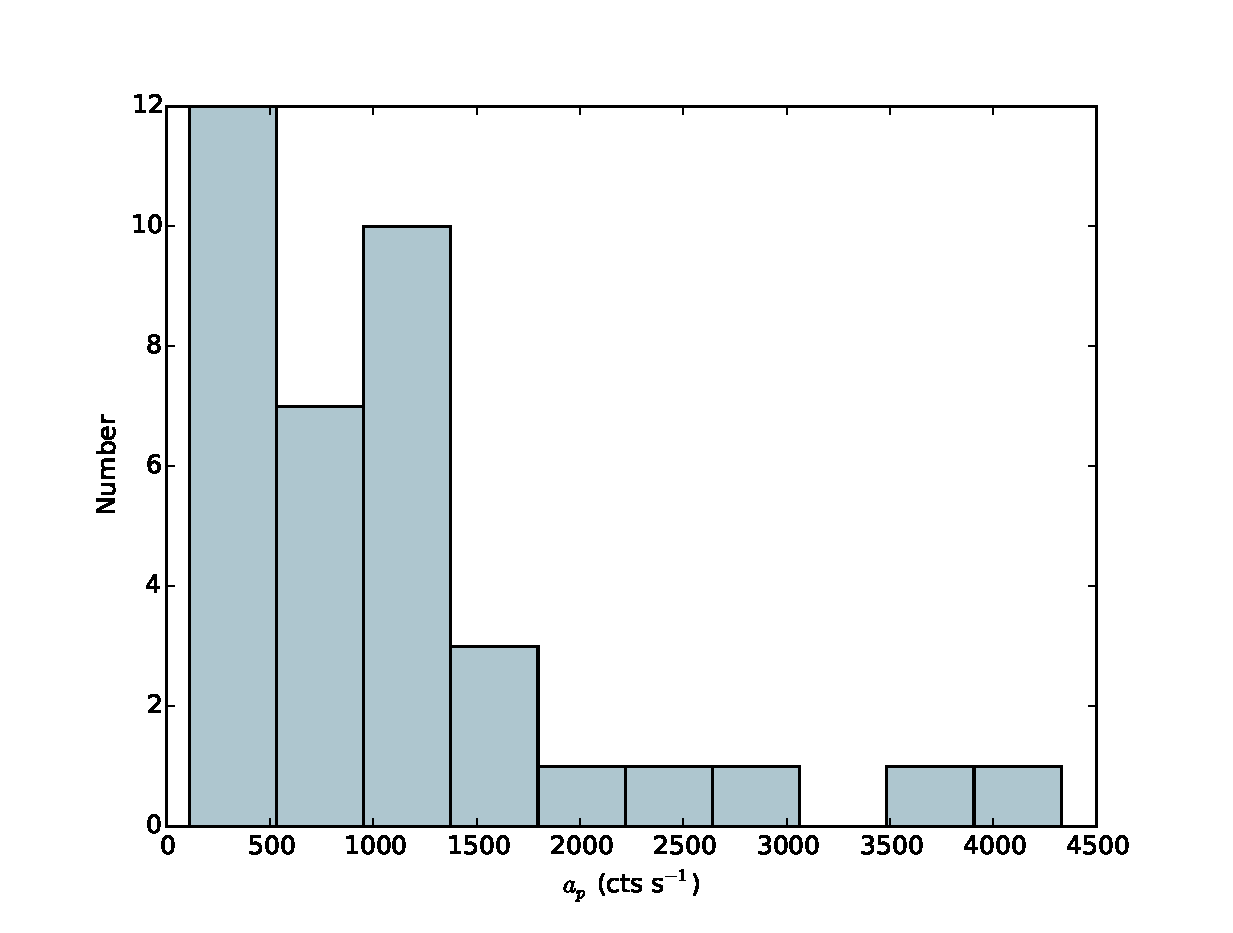
\includegraphics[width=.9\linewidth, trim={0cm 0 0cm 0},clip]{images/appendix_plat_pa_hist.eps}
  \caption{\small A histogram showing the distribution of plateau amplitude $a_p$ amongst our sample of Normal Bursts.}
  \label{fig:app_hist_ap}
\end{figure}

%-----------------

\begin{figure}
  \centering
  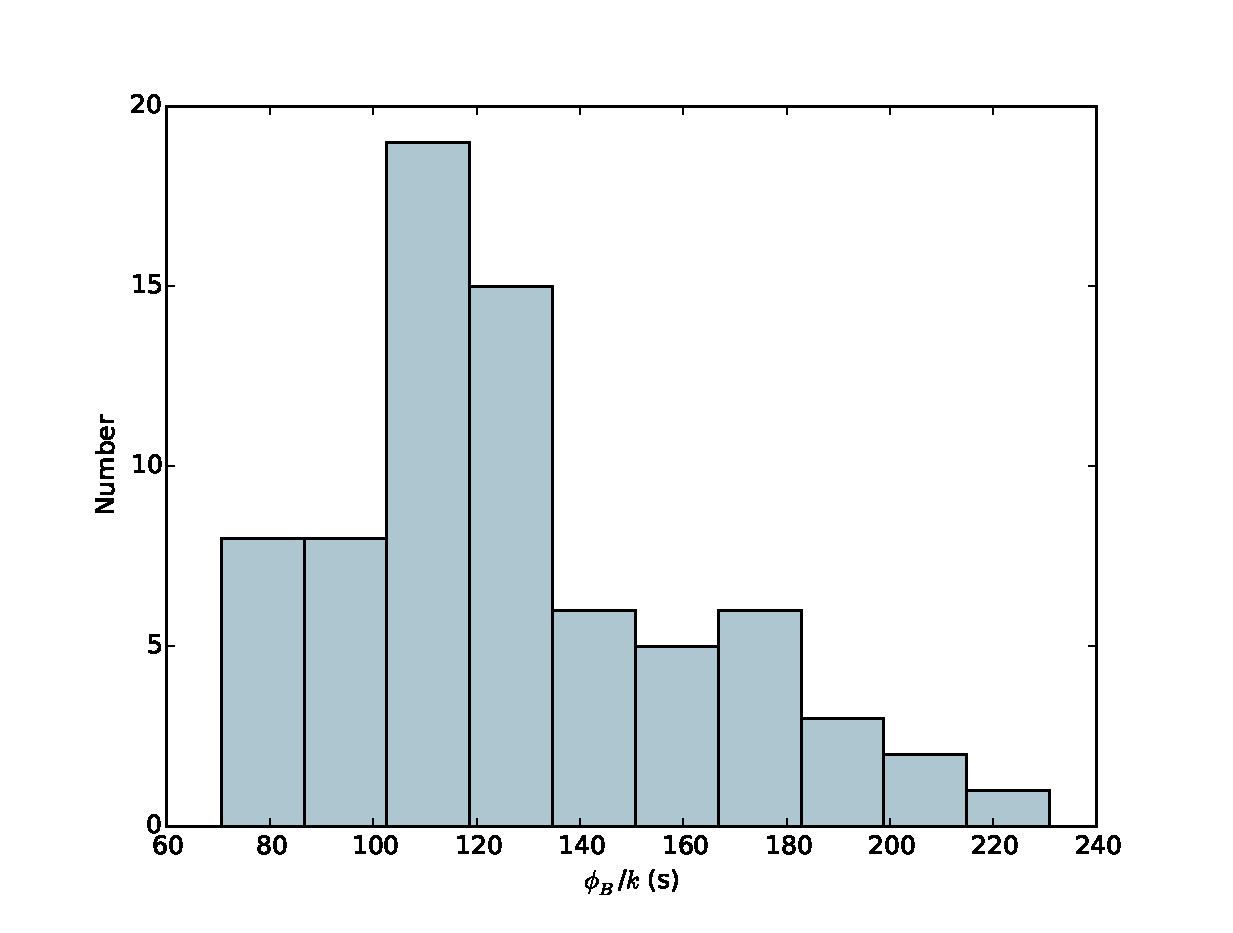
\includegraphics[width=.9\linewidth, trim={0cm 0 0cm 0},clip]{images/appendix_burst_aafluence_n_hist.eps}
  \caption{\small A histogram showing the distribution of persistent-emission-normalised burst fluence $\phi_B/k$ amongst our sample of Normal Bursts.}
  \label{fig:app_hist_phib_n}
\end{figure}

\begin{figure}
  \centering
  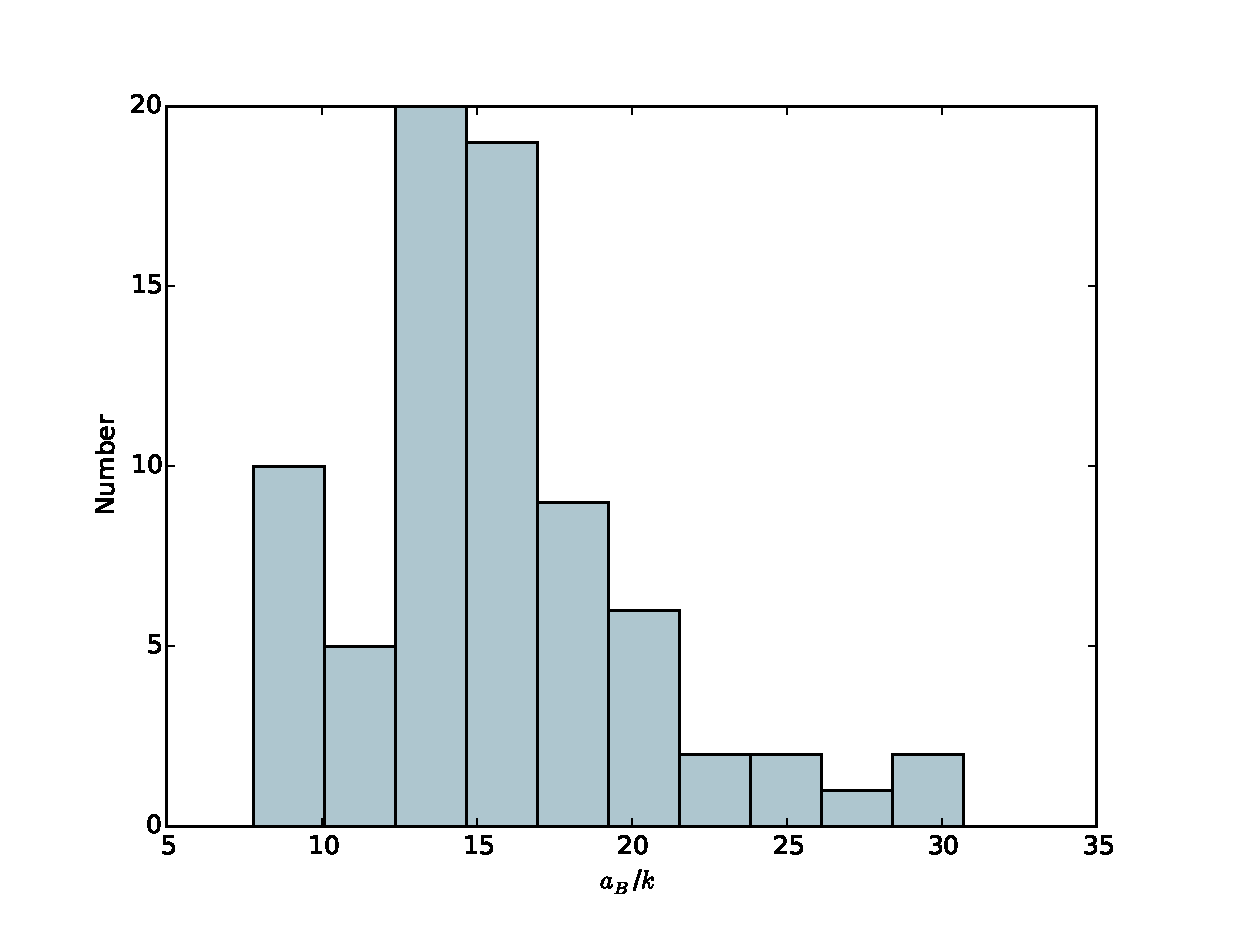
\includegraphics[width=.9\linewidth, trim={0cm 0 0cm 0},clip]{images/appendix_burst_pa_n_hist.eps}
  \caption{\small A histogram showing the distribution of persistent-emission-normalised burst amplitude $a_B/k$ amongst our sample of Normal Bursts.}
  \label{fig:app_hist_ab_n}
\end{figure}

\begin{figure}
  \centering
  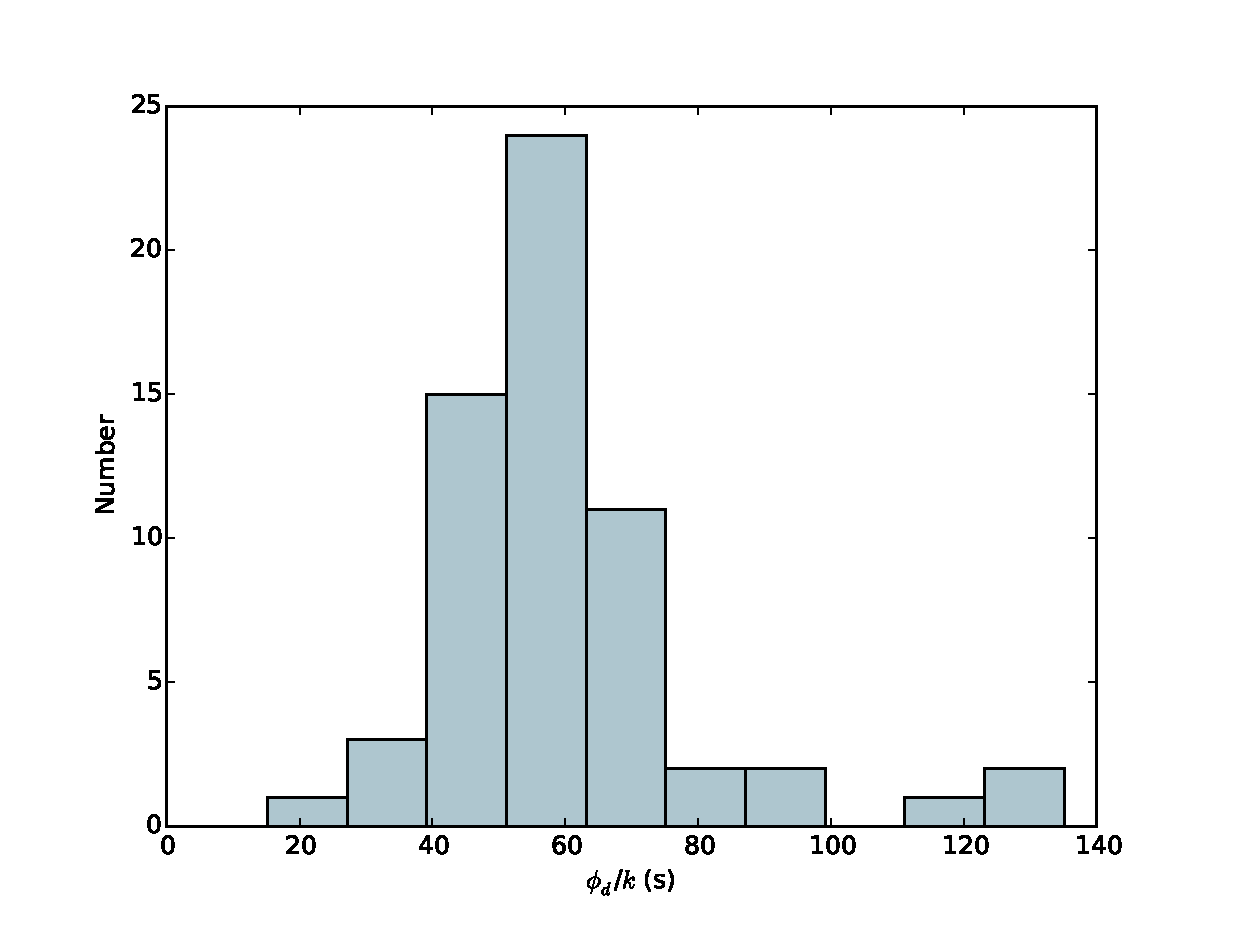
\includegraphics[width=.9\linewidth, trim={0cm 0 0cm 0},clip]{images/appendix_dip_aafluence_n_hist.eps}
  \caption{\small A histogram showing the distribution of persistent-emission-normalised dip fluence $\phi_d/k$ amongst our sample of Normal Bursts.}
  \label{fig:app_hist_phid_n}
\end{figure}

\begin{figure}
  \centering
  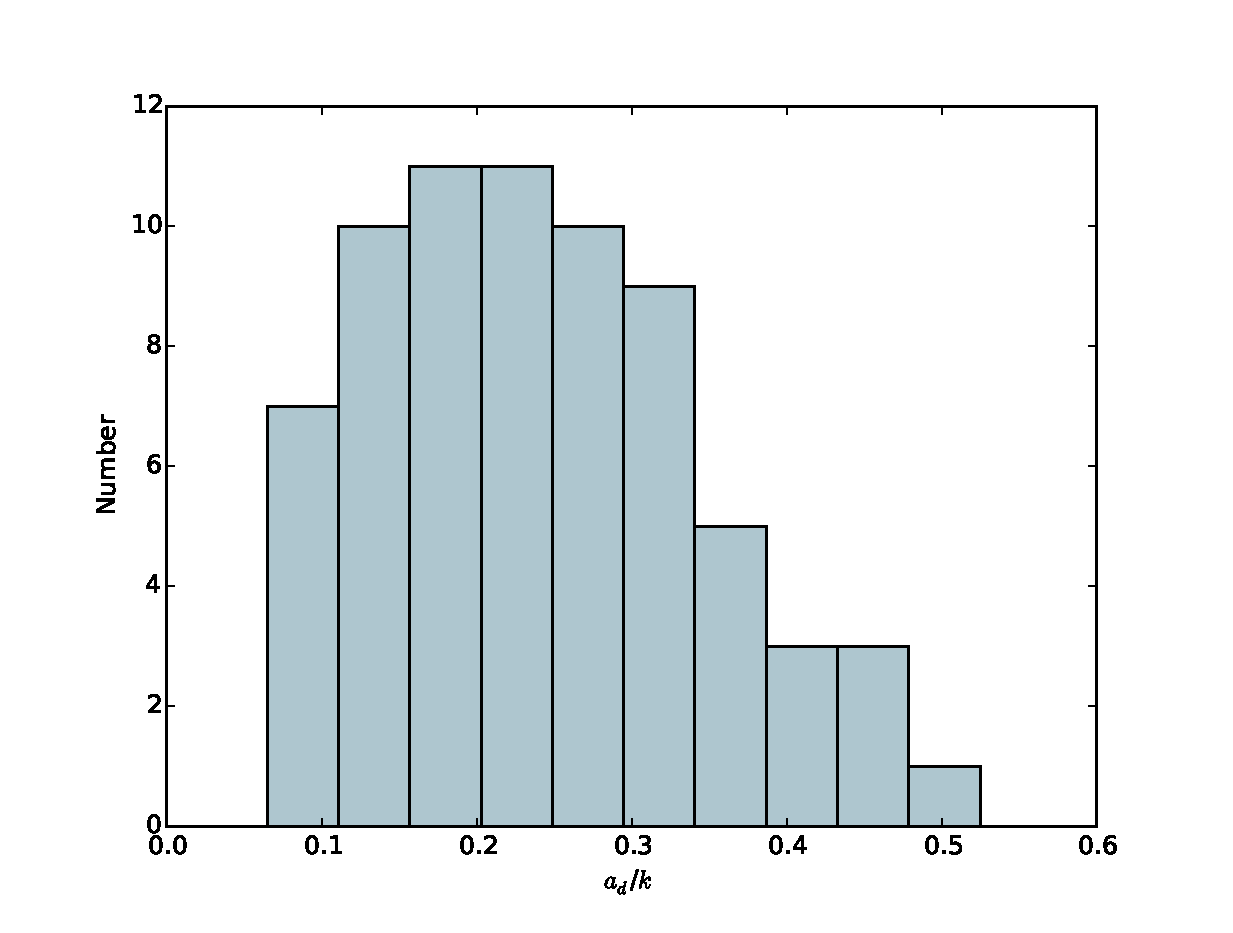
\includegraphics[width=.9\linewidth, trim={0cm 0 0cm 0},clip]{images/appendix_dip_pa_n_hist.eps}
  \caption{\small A histogram showing the distribution of persistent-emission-normalised dip amplitude $a_d/k$ amongst our sample of Normal Bursts.}
  \label{fig:app_hist_ad_n}
\end{figure}

\begin{figure}
  \centering
  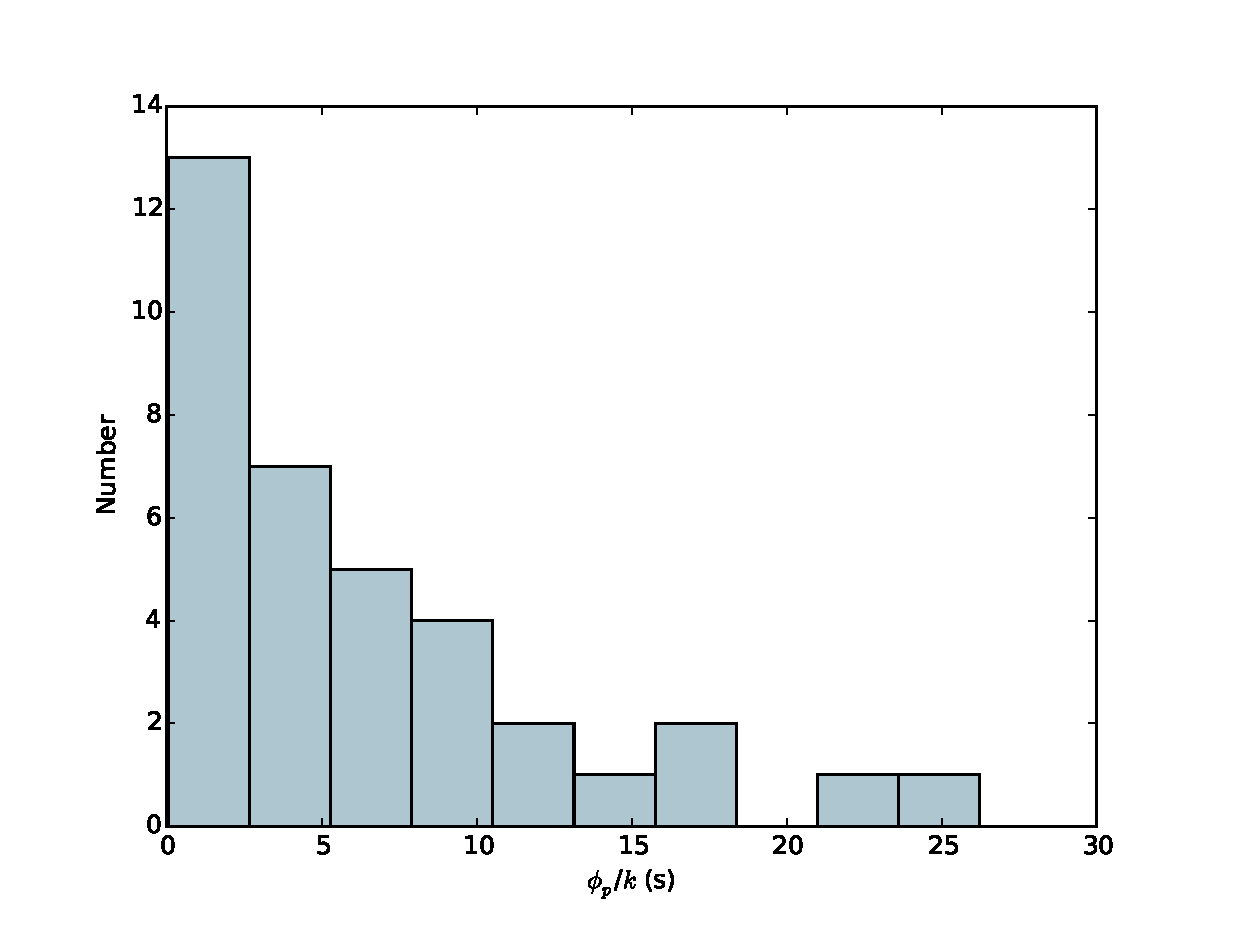
\includegraphics[width=.9\linewidth, trim={0cm 0 0cm 0},clip]{images/appendix_plat_aafluence_n_hist.eps}
  \caption{\small A histogram showing the distribution of persistent-emission-normalised plateau fluence $\phi_p/k$ amongst our sample of Normal Bursts.}
  \label{fig:app_hist_phip_n}
\end{figure}

\begin{figure}
  \centering
  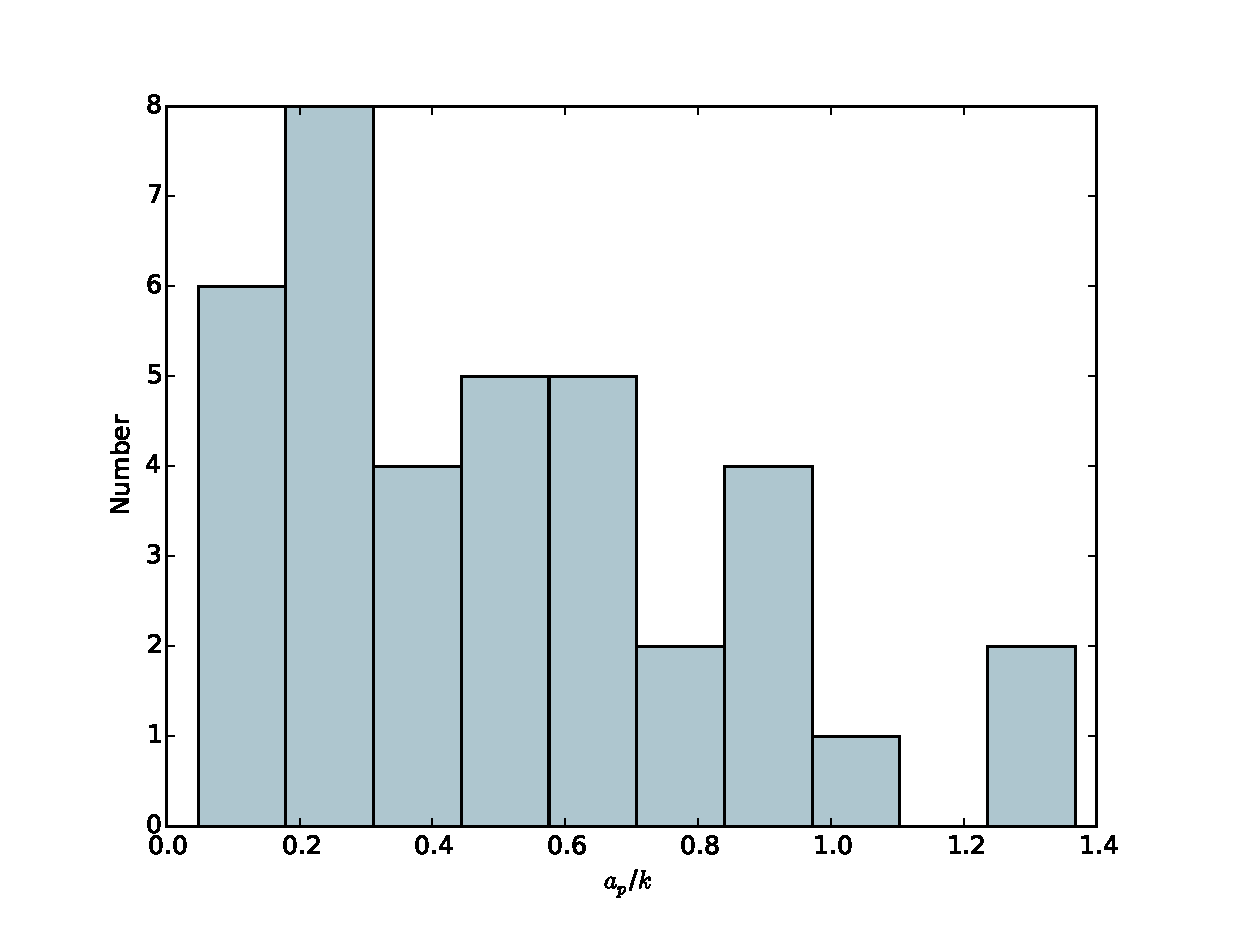
\includegraphics[width=.9\linewidth, trim={0cm 0 0cm 0},clip]{images/appendix_plat_pa_n_hist.eps}
  \caption{\small A histogram showing the distribution of persistent-emission-normalised plateau amplitude $a_p/k$ amongst our sample of Normal Bursts.}
  \label{fig:app_hist_ap_n}
\end{figure}

\section{Parameter Correlations in Normal Bursts}
\label{app:corr}

\par Before normalizing for persistent rate, we find $>5\,\sigma$ correlations between 12 pairs of the parameters we use to describe Normal Bursts:

\begin{itemize}
\item Persistent emission $k$ correlates with burst fluence $\phi_B$ ($>10\,\sigma$), burst amplitude $a_b$ ($>10\,\sigma$), dip fluence $\phi_D$ ($>10\,\sigma$) and dip amplitude $a_d$ ($7.2\,\sigma$).
\item Burst fluence $\phi_B$ also correlates with burst amplitude $a_B$ ($>10\,\sigma$), dip fluence $\phi_D$ ($>10\,\sigma$) and dip amplitude $a_d$ ($7.1\,\sigma$).
\item Burst amplitude $\phi_B$ also correlates with dip fluence $\phi_D$ ($6.2\,\sigma$) and dip amplitude $a_d$ ($5.7\,\sigma$).
\item Burst width $\sigma_B$ correlates with burst skewness $c$ ($5.8\,\sigma$).
\item Dip amplitude $a_d$ anticorrelates with dip recovery timescale $\lambda$ ($5.0\,\sigma$).
\item Plateau fluence $\phi_p$ correlates with plateau amplitude $a_p$ ($6.6\,\sigma$).
\end{itemize}

The full correlation matrix can be found in Figure \ref{fig:corr}, in which these pairs with $>5\,\sigma$ correlations are highlighted.

\begin{figure*}
  \centering
  \includegraphics[width=\linewidth, trim={2.1cm 2cm 3.5cm 3cm},clip]{images/corrplot.eps}
  \caption{\small Covariance Matrix with a scatter plot of each of the 66 pairings of the 12 Normal Burst parameters listed in section \ref{sec:NormCorr}.  Pairings which show a correlation using the Spearman Rank metric with a significance $\geq5\,\sigma$ are highlighted in red.}
  \label{fig:corr}
\end{figure*}

